\problemname{Lög um lög}
\illustration{0.3}{music}{Photo from \href{https://www.flickr.com/photos/186095195@N02/49395693758}{flickr.com}}

It occurs frequently in pop music, but also in other music genres, that the popular songs follow the same chord progression.
This gives listeners a feeling of familiarity, and therefore increases the chances that they will enjoy the song.
However, this can cause issues regarding copyright.
Because the chord progression is often the same, there is a limited amount of melodies, or the notes which are sung, to be considered.
Therefore, legal cases have popped up, in which a composer is accused of plagiarism.
The reason is that part of one song's melody sounds exactly the same as part of another song's melody.

For example, Katy Perry was sued by Marcus Gray over the song Dark Horse.
Originally, the court ruled in favour of Marcus Gray, but the verdict was overturned on the basis that the part of the melody in question was not particulary unique or rare.
It can be dangerous to set a precedent where everyone can sue everyone over a few notes.
That is why, usually, the part has to be a good portion of the song, not just a few seconds.
On occasion, it may occur, that two songs are exactly the same over a long time period and then the belief is that an act of plagiarism has been committed.
There is however the chance that it is a coincidence.
The reason for that is there are mathematics behind what tones sound nice in sequence, which composers either know or have an intuition for.

Now a record label is worried that their intellectual property is being violated.
It takes too long to listen to all the songs that might be the same, so the record label contacts you.
The request is for a program which can analyze two songs simultaneously, one from the record label and the other from the alleged plagiarizer.
The program should determine whether the songs sound similar enough to warrant legal action.
The record label is extremely worried about filing a lawsuit that would be judged in the favour of the defendant, and therefore only wants to sue
if the songs are the same in their entirety, according to music theory.

Each \emph{note}, or tone, has its own frequency. It is sufficient to set a frequency for one note and then the frequencies of the other notes may be calculated according to a rule.
An \emph{octave} is defined as the interval between two notes where one note's frequency is double the other's frequency.
In traditional European music, the octave is usually split into $12$ frequencies which are in sequence, and are called the chromatic scale,
with an equal interval from one note to the next which is named \emph{semitone} or \emph{half step}.
A \emph{whole step} is then two half steps.
On a piano you can see these twelve tones, repeated, once in each octave, but usually with incomplete octaveson the far left and the far right.

\begin{figure}[ht!]
  \centering
    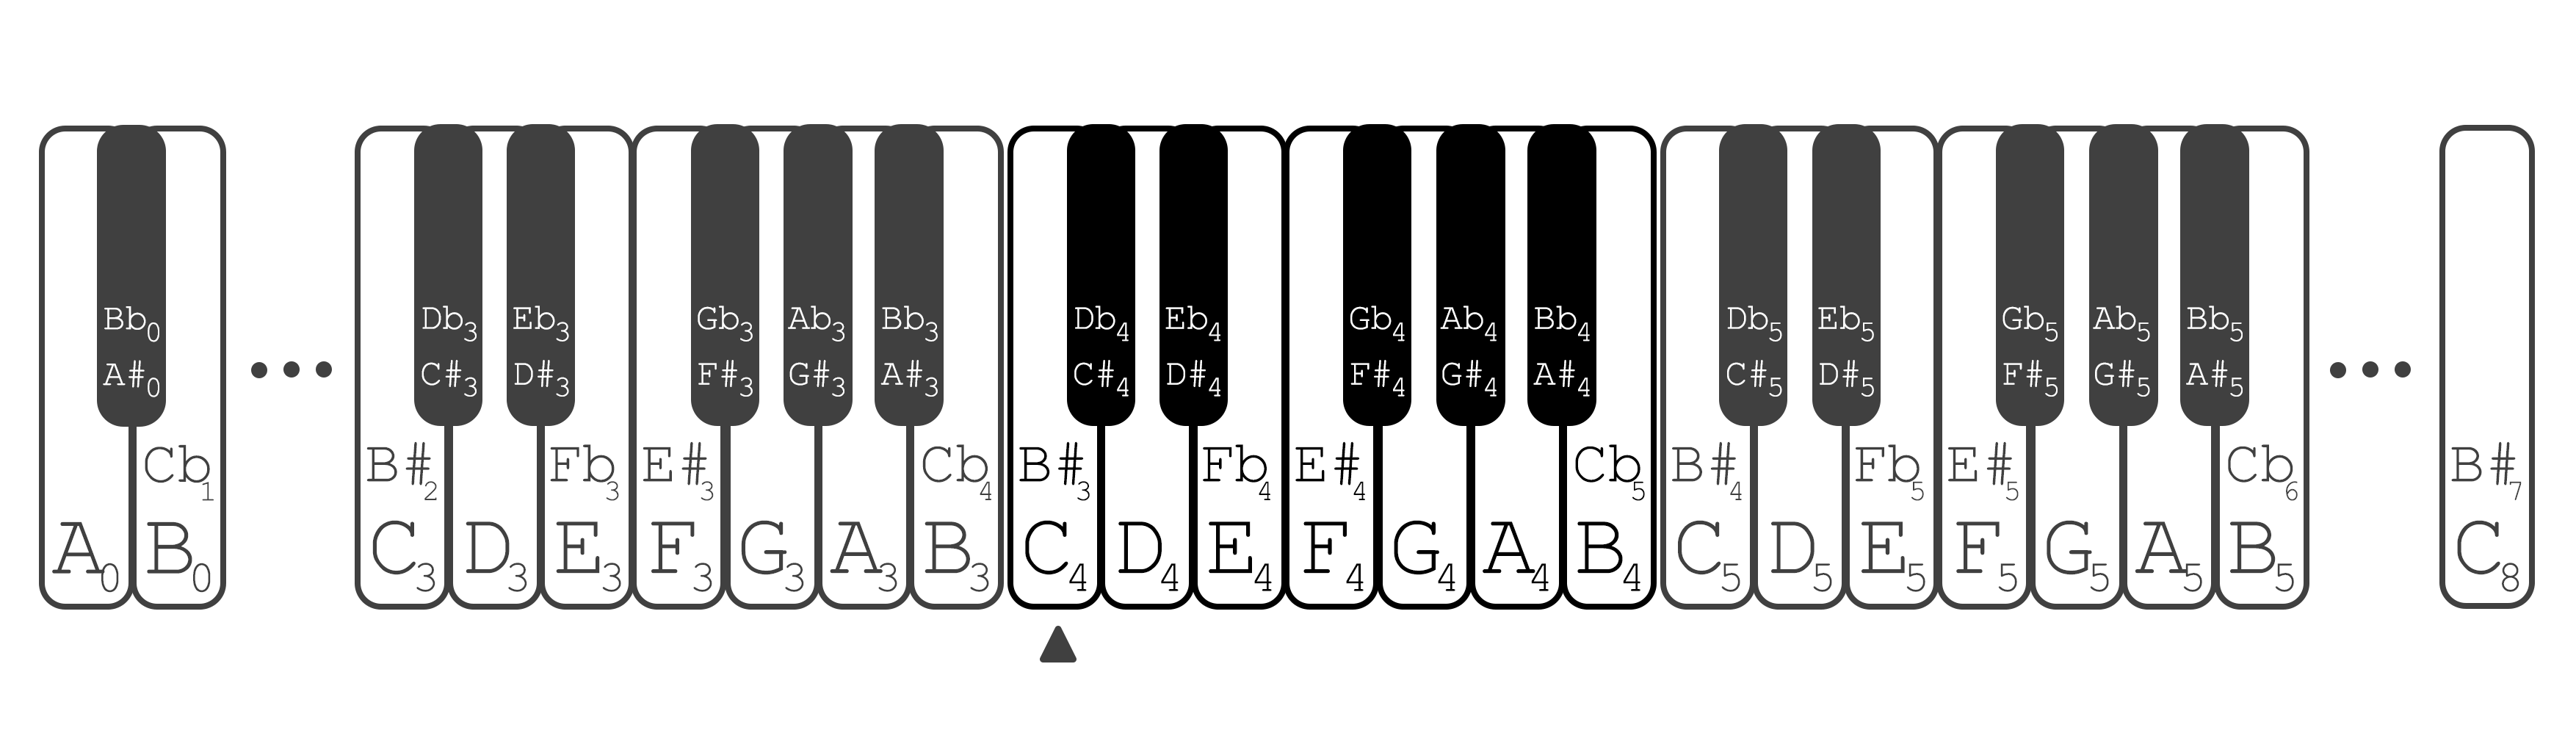
\includegraphics[width=0.9\textwidth]{piano}
  \caption{Notes marked on the keys of a piano.}
\end{figure}

Pianos are designed around the seven tone major scale, specifically \texttt{C} major.
The base note is then \texttt{C} and the scale follows the formula:
whole step, whole step, half step, whole step, whole step, whole step, half step.
The notes are named after the letters \texttt{A-G}, as can be seen in the image, and the \texttt{C} major scale consists of the notes \texttt{C D E F G A B}, which correspond to the white keys on the piano.
The notes which are not in the \texttt{C} major scale are exactly the notes corresponding to the black keys on the piano.
They are named based on the other notes with additional half steps up or down.
A half step up is written by adding \texttt{\#} after the note, but a half step down is written by adding a \texttt{b} after the note.
Therefore the notes in an octave are \texttt{C C\#/Db D D\#/Eb E F F\#/Gb G G\#/Ab A A\#/Bb B}, but also note that one can write \texttt{Cb} for \texttt{B}, \texttt{B\#} for \texttt{C}, \texttt{Fb} for \texttt{E} and \texttt{E\#} for \texttt{F}.
To signify on which octave each note is being played, an integer is added to the back of the note.
The octaves are in increasing order from left to right and the first \texttt{C} note marks the start of octave $1$.
If the fourth octave were written up in its entirety it could be written as \texttt{C4 C\#4 D4 D\#4 E4 F4 F\#4 G4 G\#4 A4 A\#4 B4}.
The note on the far left on an $88$ key piano is \texttt{A0}, the note known as middle \texttt{C} is \texttt{C4}, marked by a triangle in the image, and the note on the far right is \texttt{C8}.

Melodies are a big part of songs and they can be defined as a series of notes and rests.
Rests are symbolized by \texttt{-} and represent the absence of sound.
Each note or rest lasts for the same amount of time.
To determine whether two songs are the same you can use the following rules:

\begin{itemize}
    \item Rule 1: If two melodies are written exactly the same, then they represent the same song.
    For example, the melodies \texttt{C4 D4 - E4} and \texttt{C4 D4 - E4} are the same.
    \item Rule 2: If two melodies are written differently, but the notes are equivalent, then they represent the same song.
    For example, the melodies \texttt{C4 C\#4 - Eb4} and \texttt{B\#3 Db4 - D\#4} are the same.
    \item Rule 3: If two melodies are written the same, except all the notes in one of them have been transposed, or shifted, by the same number of octaves, then they represent the same song.
    For example, the melodies \texttt{B3 D4 - E4} and \texttt{B5 D6 - E6} are the same.
    \item Rule 4: If two melodies are written the same, except all the notes in one of them have been transposed, or shifted, by the same number of semitones, then they represent the same song.
    For example, the melodies \texttt{B3 D4 - E4} and \texttt{C\#4 E4 - F\#4} are the same.
\end{itemize}

If the songs have not been determined to be the same after the application of these rules, then the songs are not the same.

\section*{Input}
Input starts with one line containing a positive integer $n$, where $1 \leq n \leq 10^5$, which represents the length of each melody.
Next two lines follow, each with a melody, where the melodies consist of $n$ values representing notes or rests, separated by spaces.
Notes and rests are written in the same form as mentioned previously in the statement.
The lowest note appearing in the input is \texttt{A0} and the highest note is \texttt{C8}, corresponding to an $88$ key piano.
Each note will have a maximum of one \texttt{\#} symbol or \texttt{b} symbol.


\section*{Output}
Output \texttt{Jebb} if the songs are the same, and the record label should sue, otherwise output \texttt{Neibb}.

\section*{Scoring}
\begin{tabular}{|l|l|l|}
\hline
Group & Points & Constraints \\ \hline
1     & 15     & Rule $1$ is required \\ \hline
2     & 25     & Rules $1$ and $2$ are required \\ \hline
3     & 15     & Rules $1$ and $3$ are required \\ \hline
4     & 10     & Rules $1$, $2$ and $3$ are required \\ \hline
5     & 35     & All rules are required \\ \hline
\end{tabular}

\section*{Additonal info on samples}
To listen to the melodies in the sample inputs, you can download the sound files \href{/problems/iceland.logumlog/file/statement/attachments/melodies.zip}{here}.
In sample $5$ you can hear parts of melodies from the songs Ég Á Líf by Örlygur Smári, the former melody, and I Am Cow by the band The Arrogant Worms, the latter melody.
In sample $8$ you can hear two parts of the melody from the song Paradise Lost by Symphony X, where the latter melody is the same as the former, but transposed up by a whole step.

